%%% Local Variables:
%%% mode: latex
%%% TeX-master: "mu2e-36575"
%%% End:

%%%%%%%%%%%%%%%%%%%%%%%%%%%%%%%%%%%%%%%%%%%%%%%%%%%%%%%%%%%%%%%%%%%%%%%%%%%%% 
\section{Track Selections}

Selection of correctly reconstructed tracks plays a critical role in the search.
In the Mu2e offline, there are two track fitters which correspond to two different
hit ambiguity resolvers. An ANN-based training has been performed only for one of them,
so-called ``panel-based ambiguity resolver''.

We performed a similar training for the output of the track fits using the doublet-based
ambiguity resolver.

Following \cite{MU2E_4595_ANN_TRAINING}, we used ROOT TMVA package to train a MLP ANN
with 8 input variables and one hidden layer. The following variables were used as inputs:

.....

The goal of training was to optimize separation of the electron tracks reconstructed correctly,
with $\Delta{P} = |P_{reco}-P_{true}| < 0.25$ MeV/c, or approximately $2\sigma$, from tracks
reconstructed with $\Delta{P} > 0.7$ MeV/c, or , approximately, $5\sigma$ above the true value.
The comparison between the $P_{true}$ and $P_{reco}$ was performed in a plane corresponding to
the tracker entrance. 

As a cross-check, we also trained a BDT-based TMVA classifier. Similar to \cite{MU2E_33150_ANN_TRAINING},
we found that the ANN performed slightly better, so current analysis uses an ANN-based track
quality selection.

\begin{figure}
\begin{tikzpicture}
  \node[anchor=south west,inner sep=0] at (0,0.) {
    % \node[shift={(0 cm,0.cm)},inner sep=0,rotate={90}] at (0,0) {}
    % \makebox[\textwidth][c] {
      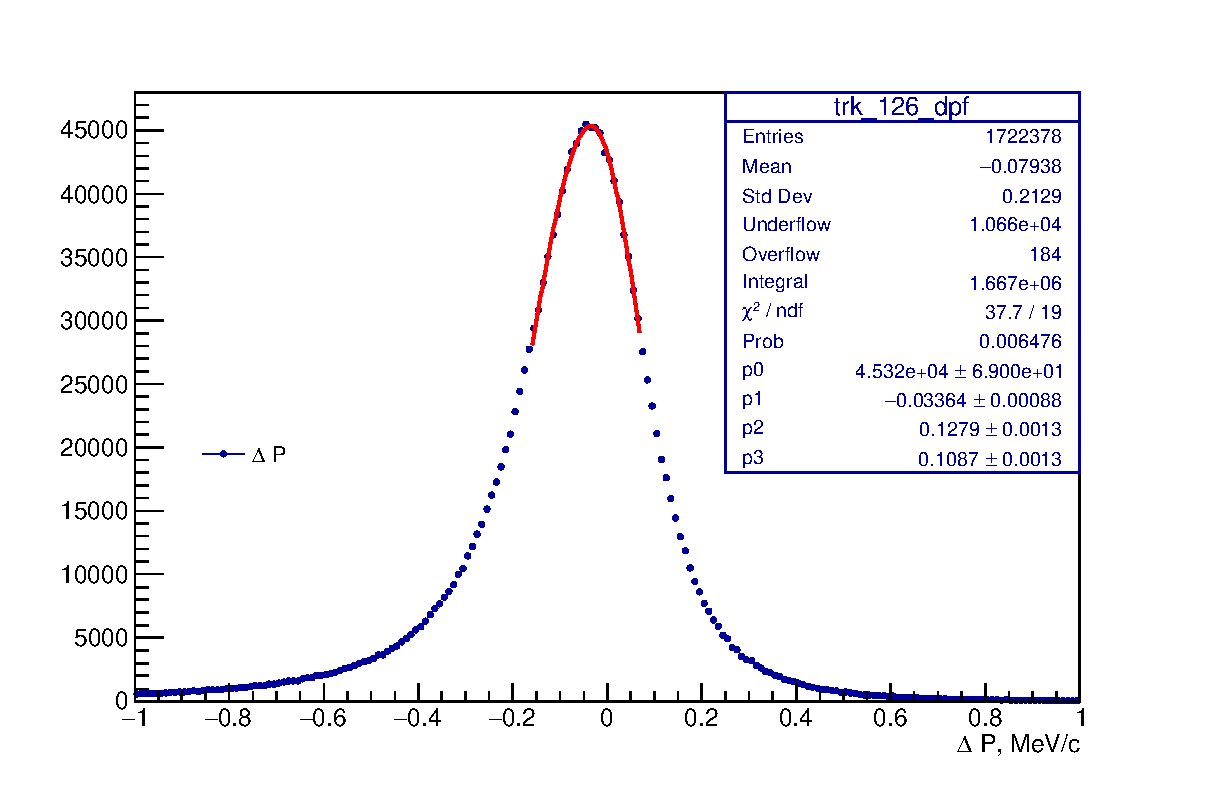
\includegraphics[width=0.55\textwidth]{figures/pdf/figure_00112_fele2s51b1_track_comp_ffff_1070_nocorr_trk_126_dpf}
    %}
  };
  \node[anchor=south west,inner sep=0] at (8,0.) {
    % \node[shift={(0 cm,0.cm)},inner sep=0,rotate={90}] at (0,0) {}
    % \makebox[\textwidth][c] {
      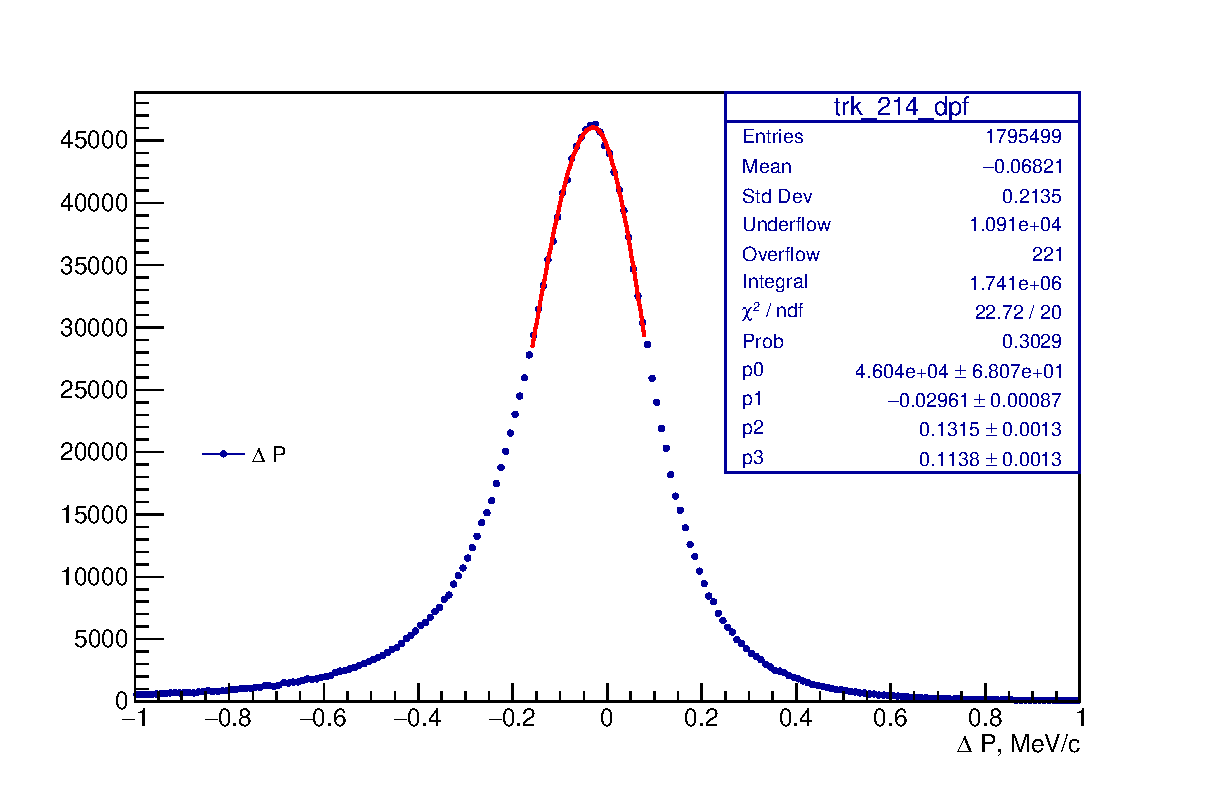
\includegraphics[width=0.55\textwidth]{figures/pdf/figure_00113_fele2s51b1_track_comp_ffff_1070_nocorr_trk_214_dpf}
    %}
  };
  % \node [text width=6cm, scale=0.8] at (4.5,6.4) {mu2e-18894 by Kevin Lynch and Jim Popp};
\end{tikzpicture}

\caption{
  \label{fig:sindrum_ii_fig_08_fit} 
  $\Delta P$ distributions at the tracker front for PAR (left) and DAR (right) tracks. The distributions  
  are fit with the asymmetric ($\sigma_{left} \ne \sigma_{right}$) gaussian function. Peak positions are used
  to correct the reconstructed  momenta of the tracks coming of the respective fits.
}
\end{figure}


Improvements in the track reconstruction resulted in a significantly better separation
between the two classes of tracks. For example, the expected relative contribution of
the DIO tracks with $\Delta{P} > 0.5$ MeV inthe ``signal'' region, [103.6,105.0] MeV/s was
found to be 0.228. This number is 50\% lower than 0.355, estimated in \cite{MU2E_4595_ANN_TRAINING}
for the same region.
\begin{figure}
\begin{tikzpicture}
  \node[anchor=south west,inner sep=0] at (0,0.) {
    % \node[shift={(0 cm,0.cm)},inner sep=0,rotate={90}] at (0,0) {}
    \makebox[\textwidth][c] {
      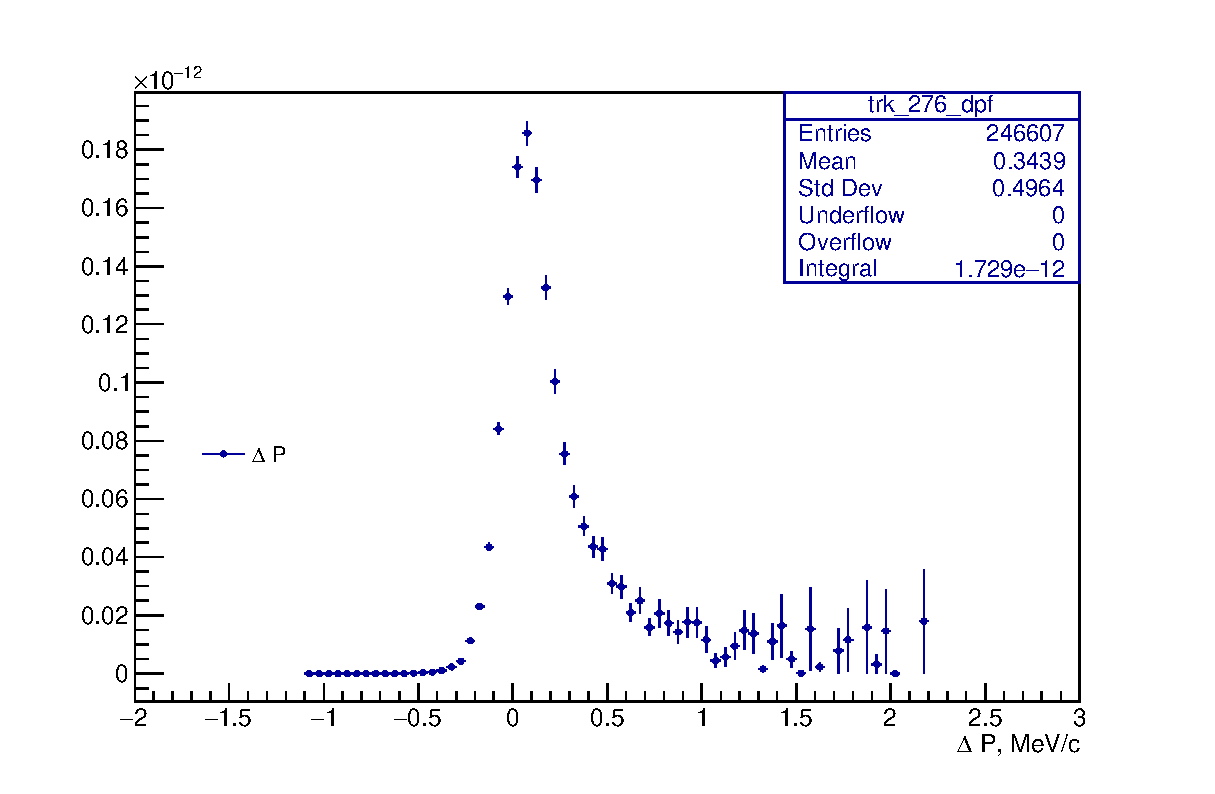
\includegraphics[width=0.99\textwidth]{figures/pdf/figure_00111_fele2s51b1_track_comp_ffff_1070_trk_276_dpf}
    }
  };
  % \node [text width=6cm, scale=0.8] at (4.5,6.4) {mu2e-18894 by Kevin Lynch and Jim Popp};
\end{tikzpicture}
% \captionof{figure} {
\caption{
  \label{fig:sindrum_ii_fig_08_fit} 
  $\Delta P ~=~ P_{reco} -P_{true}$ distribution for simulated DIO background in the region [103.6,105.0] MeV.
  77.2\% of reconstructed events in this region are expected to have $\Delta P < 0.5$ MeV/c
}
\end{figure}

To explore the parameter space, we also trained a similar ANN to discriminate the tracks for
$\Delta{P} < 0.25$ MeV/c from tracks with $\Delta{P} > 0.6$ MeV/c. No improvement in the DIO
suppression in the region [103.85, 104.9] MeV/c was observed. 

To choose between the PAR-based and DAR-based fitters, we compared performance of the
trained DAR ANN to the performance of the PAR ANN.

The results are shown in Figure ..... .
Using the CD3 choice of the signal region , 103.85 < p < 104.9 MeV/c, we compared the
CE reconstruction efficiency of the two methods vs the expected DIO background.

The relative efficiency is 